\documentclass[10pt,a4paper,twocolumns]{article}
%==================================================================

\usepackage{acteja}

\usepackage{nidanfloat}

%% \actejaset is for editors only
%% \actejaset{VOL}{NO}{YEAR}{from}{to}{articlenumber}{headerstring}
\actejaset{XX}{Y}{20XX}{0}{0}{ZZZ}{A. Author et al.}
%==================================================================


\title{Formal Requirements for the Papers Submitted to the ``Acta Technica Jaurinensis'' Periodical}

\author{Firstname Surname$^1$$^,$$^*$, Firstname Surname$^1$, Firstname Surname$^2$}

\institute{
$^1$Name of the Department, Name of the University\\
Address, Zip code Cite, Country \\

$^2$Name of the Institute\\
Address, Zip code City, Country \\

$^*$e-mail: corresponding\_author@email.address}

%  \institute is not a standard element of LaTeX titles, but
%  helps us to produce the same formatting. Please, use it

\begin{document}

\twocolumn[  
    \begin{@twocolumnfalse}
        
\maketitle

\centerline{\begin{footnotesize}Submitted: Day/Month/Year; Accepted: Day/Month/Year; Published online: Day/Month/Year\end{footnotesize}}

\begin{abstract}
These instructions give you guidelines for preparing manuscripts for the ACTA TECHNICA JAURINENSIS journal. Use this document as a template if you are using Microsoft Word 13 or later. Otherwise, use this document as an instruction set. Define all symbols used in the abstract. Do not cite references in the abstract. The length of the abstract must be at least 150 words and maximum 250 words.
\end{abstract}

\keywords{Minimum 3 maximum 5 key words or phrases in alphabetical order, separated by semicolons}

     \end{@twocolumnfalse}
]

%----------------------------------------------------------------------------


\section{Introduction}

Acta Technica Jaurinensis is a peer reviewed scientific journal published by the Széchenyi István University, Győr. It was founded in 2008. The journal is published on terminally. The main scope of Acta Technica Jaurinensis is to provide a publication possibility related to the following topics: vehicle, mechanical engineering and mechatronics; transportation science and logistics; architecture, civil and agricultural engineering; information technology and electrical engineering. We are ready to publish any short original publication, new research result as well as review articles covering broader topics. The subject matter can be theory, methodology, empirical studies and applications.

Each paper is evaluated in a blind peer review process. The journal is electronically published and indexed. It is an open access journal, both downloading the published articles and publication is free of charge. The users have the right to read, print, search, download, copy, distribute or link to the full texts of these articles, given that they credit the original source, without any alterations or commercial use.


\section{Methods}

The name(s) of the author(s) has/have to be given in the following way: whole first name and whole surname. Please avoid adding the different titles of the author(s). In the header, author names are expected in the ``C. Surname'' format where ``C'' is the initial of the first name. In the case of 2 authors give the names of each author, between the names use "and", over 3 authors give the names of the first authors, then use the expression "et al.".

Do not format anything in the paper, use only predefined styles, and do not add any new style. There is only one exception: tables can only be formatted individually using Microsoft Word’s “format table”.

\section{Examples of the elements of a document}

\subsection{Placing figures and tables in the text}

In case of placing figures and tables use a Text Box. The text box includes the figure or table and its caption. The text box fitting must be square type in the “wrap text” option. Normally the width of figures and tables must not be wider than 7 cm to fit in a column. If it is necessary to use wider tables or figures, it can be used 15.5 cm wide, but in this case it must be fit to the top or the bottom of the page like Table 2.

\subsubsection{Placing images, figures in the text}

Insert pictures, images and figures in a separate paragraph. The caption should be numbered manually, according to the pattern shown in
\textbf{Fig. \ref{fig:figure1label}}. In the text box, the caption name must be full (i.e. Figure 1) but in the text reference, it must be in short form (i.e. Fig. 1). The resolution should be at least $300$ dpi.

\begin{figure}[htbp]
\begin{center}
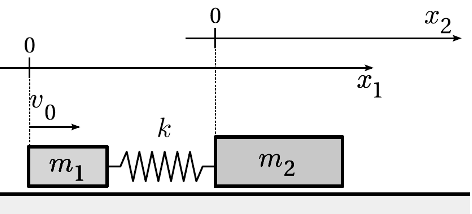
\includegraphics[width=0.4\textwidth]{fig/slbp-bodies.png}
\end{center}
\caption{Figure caption.}
\label{fig:figure1label}
\end{figure}


\subsubsection{Tables in the text}

The table should be centered, and the relevant caption should be placed above the table (see \textbf{Table \ref{tab:table1label}}). Tables should be as simple as possible. Do not use picture for tables. Do not forget to use table caption style.


\begin{table}[htbp]
\centering \caption{Table caption}\label{tab:table1label}
\begin{tabular}{c c c} \hline
 \textbf{\emph{Column A}} &\textbf{\emph{Column B}} & \textbf{\emph{Column C}} \\ \hline
  100 \%  	&	50 		&	2 \\
  90 \%  	&	38 		&	4 \\
  80 \%  	&	34 		&	0 \\
  70 \%  	&	20 		&	2 \\ \hline
\end{tabular}
\end{table}

\subsection{Formulas in the text}

The following conventions should be taken into account.

\begin{itemize}
    \item Formulas and mathematical symbols should be created with an equation/formula editor, and should be numbered manually.
    \item Do not use picture for equations.
    \item Formulas should be written in a consistent manner throughout the whole document.
    \item Do not use the letter x as a sign of multiplication (as it is the sign of the Cartesian product).
\end{itemize}

\begin{table*}[b]
\centering \caption{Table caption}\label{tab:table2label}
\begin{tabular}{c c c c c c c c} \hline
 \textbf{\emph{Column A}} &\textbf{\emph{Column B}} & \textbf{\emph{Column C}} & \textbf{\emph{Column D}} & \textbf{\emph{Column E}} & \textbf{\emph{Column F}} & \textbf{\emph{Column G}} & \textbf{\emph{Column H}} \\ \hline
  100 \%  	&	50 		&	2 &	2 &	2 &	2 &	2 &	2 \\
  90 \%  	&	38 		&	4 &	2 &	2 &	2 &	2 &	2 \\
  80 \%  	&	34 		&	0 &	2 &	2 &	2 &	2 &	2 \\
  70 \%  	&	20 		&	2 &	2 &	2 &	2 &	2 &	2 \\ \hline
\end{tabular}
\end{table*}

Numbers should have normal (not italic) format in the formula. You can see some examples of equations (\ref{eq:01}) to (\ref{eq:03}).

\begin{equation}\label{eq:01}
  (x+a)^n=\sum_{k=0}^{n} \binom{n}{b} x^{k} a^{n-k}
\end{equation}

\begin{equation}\label{eq:02}
  x=\frac{-b\pm\sqrt{b^2-4ac}}{2a}
\end{equation}

\begin{equation}\label{eq:03}
  \cos \alpha + \cos \beta = 2 \cos \frac{1}{2}(\alpha + \beta) \cos \frac{1}{2}(\alpha - \beta)
\end{equation}

\subsection{References in the text}

The author(s) takes/take the full responsibility for the accuracy of their references. The format of references must be uniform and consistent with the instructions below. All publications cited in the text should be referred to by a number in square brackets (e.g., \cite{article_a}). Concatenation of references (e.g., [1-4]) is not allowed. Note that only one reference belongs to one number. Use “Cite” style for left alignment and automatic numbering. All doi numbers should be represented if available, and use “Shift – Enter” keys for new line break.

The examples of references of papers in English \cite{article_a}, papers in other languages \cite{article_b}, books \cite{book}, book chapters \cite{incollection}, conference proceedings \cite{conference}, theses \cite{phdthesis}, standards \cite{standard}, patents \cite{patent} and online \cite{online} are shown in References. If the page numbering of the journal is not continuous within one year, the article ID should be given instead of the page numbers \cite{article_c}. The doi number and URL must be hyperlinks \cite{article_a} \cite{book} \cite{conference} according to Link style.

In the list of references author names are expected in the "C. Family" format where "C" is the initial of the first name. Till there are 3 authors, give the names of each author \cite{article_b}, over 3 authors give the names of the first 2 authors, then use et al. \cite{article_d}. Provide the complete title of publication (title of paper, book, book chapter, standard, patent). Do not abbreviate journal or conference names, e.g. write "Transactions on Medical Imaging" instead of "Trans Med Imaging".

\section*{Acknowledgement}
The publishing of this paper was supported by XY.

\section*{Author contributions}

\paragraph{A. Author:} Conceptualization, Experiments, Theoretical analysis.
\paragraph{B. Author:} Finite element modelling, Writing, Review and editing.
\paragraph{C. Author:} Supervision, Review and editing.

\section*{Disclosure statement}
The authors declare that they have no known competing financial interests or personal relationships that could have appeared to influence the work reported in this paper.

\section*{ORCID}

If the authors have ORCID identification, it may be given in this section.
Firstname Surname http://orcid.org/0000-0000-0000-0000
Firstname Surname http://orcid.org/0000-0000-0000-0000


%%%%%%%%%%%%%%%%%



%----------------------------------------------------------------------------



%----------------------------------------------------------------------------


\begin{thebibliography}{1}

\bibitem{article_a}
V.~A. Szabó, G.~Dogossy, Recycling of mineral water bottles with chemical
  foaming,  \textit{Acta Technica Jaurinensis} 10~(2) (2017) pp. 157--167.
	\newline doi: \begin{footnotesize}\url{https://doi.org/10.14513/actatechjaur.v10.n2.446}\end{footnotesize}

\bibitem{article_b}
E.~Turfa, G.~Dogossy, F.~Ronkay, Improvement of recycled pet properties by
  reactive extrusion,  \textit{Anyagok Világa} 11~(2) (2013) pp. 50--58, in Hungarian.

\bibitem{book}
M.~Kuczmann, A.~Iványi, The Finite Element Method in Magnetics, 1st Edition,
  Akadémiai Kiadó, Budapest, 2008.
	\newline doi: \begin{footnotesize}\url{https://doi.org//10.13140/2.1.3104.1927}\end{footnotesize}

\bibitem{incollection}
M.~Kuczmann, Identification of isotropic and anisotropic vector preisach model,
  in: A.~Iványi (Ed.), Preisach Memorial Book: Hysteresis models in
  mathematics, physics and engineering, 1st Edition, Akadémiai Kiadó,
  Budapest, 2005, pp. 89--102.

\bibitem{conference}
A.~Kovács, G.~Lencse, Modelling of virtualized servers, in: N.~Herencsár,
  K.~Molnár (Eds.), 38th International Conference on Telecommunications and
  Signal Processing: TSP 2015, Brno University of Technology, Brno, 2015, pp.
  241--245.
	\newline doi: \begin{footnotesize}\url{https://doi.org/10.1109/TSP.2015.7296260}\end{footnotesize}


\bibitem{phdthesis}
V.~Nagy, Examination and modeling of porosity in polyester twisted fibrous
  structures, Ph.D. thesis, Budapest University of Technology and Economics
  (2006).
	\newline URL \begin{footnotesize}\url{http://hdl.handle.net/10890/467}\end{footnotesize}

\bibitem{standard}
Plastics -- determination of tensile properties -- part 1: General principles,
  {ISO 527-1:2012} (2012).

\bibitem{patent}
M.~Horski, Brushless motor with inside mounted single bearing, {US 5654598 A}
  (1997).

\bibitem{online}
CostumPartNet,
  \href{http://www.custompartnet.com/wu/InjectionMolding}{Injection molding}
  [cited 2018-01-24].
\newline URL \begin{footnotesize}\url{http://www.custompartnet.com/wu/InjectionMolding}\end{footnotesize}

\bibitem{article_c}
L.~Lendvai, I.~Sajó, J.~Karger-Kocsis, Effect of Storage Time on the Structure and Mechanical Properties of Starch/Bentonite Nanocomposites,  \textit{Starch-Starke} 71~(1-2) (2019) 1800123.
\newline doi: \begin{footnotesize}\url{https://doi.org/10.1002/star.201800123}\end{footnotesize}
	
	\bibitem{article_d}
M.~Gáspár, Z.~Benkő et al., Reducing water absorption in compostable starch-based plastics, 
 \textit{Polymer Degradation and Stability} 90~(3) (2005) pp. 563--569.
\newline doi: \begin{footnotesize}\url{https://doi.org/10.1016/j.polymdegradstab.2005.03.012}\end{footnotesize}

\end{thebibliography}


\begin{table}[H]

\begin{minipage}{.15\textwidth}
    \begin{tabular}{*{1}{p{0.15\textwidth}}}
\includegraphics[height=5.5mm]{\cc}
\\
\end{tabular}
\end{minipage}% 
\begin{minipage}{.5\textwidth}
    \begin{tabular}{*{1}{p{0.5\textwidth}}}
\footnotesize 
This article is an open access article distributed under the terms and conditions of the Creative Commons Attribution NonCommercial (\href{https://creativecommons.org/licenses/by-nc/4.0/}{CC BY-NC 4.0}) license. \\
\end{tabular}
\end{minipage}%
\end{table}


\end{document}